\documentclass[a4paper,11pt]{article}

\usepackage[utf8]{inputenc}
\usepackage[T1]{fontenc}
\usepackage{lmodern}
\usepackage{textcomp}
\usepackage[a4paper,margin=2.6cm]{geometry}
\usepackage[table]{xcolor}   % caricato UNA sola volta, prima di tcolorbox
\usepackage{graphicx}
\usepackage{float}
\usepackage{booktabs}
\usepackage{amsmath}
\usepackage{siunitx}
\usepackage{listings}
\usepackage{enumitem}
\usepackage{caption}
\usepackage{titlesec}
\usepackage{fancyhdr}
\usepackage{tcolorbox}
\usepackage{array}
\usepackage{longtable}
\usepackage{parskip}
\usepackage{hyperref}        % hyperref va caricato per ultimo

% ----- Colors -----
\definecolor{bluepoli}{cmyk}{0.4,0.1,0,0.4}
\definecolor{lightbluepoli}{RGB}{235,242,250}
\definecolor{todobg}{RGB}{248,248,248}
\definecolor{todoframe}{RGB}{180,180,180}

% ----- Hyperref -----
\hypersetup{
    colorlinks=true,
    linkcolor=bluepoli,
    urlcolor=bluepoli,
    citecolor=bluepoli
}

% ----- Section style -----
\titleformat{\section}
{\color{bluepoli}\normalfont\Large\bfseries}
{\thesection}{0.8em}{}

\titleformat{\subsection}
{\color{bluepoli}\normalfont\large\bfseries}
{\thesubsection}{0.8em}{}

\titleformat{\subsubsection}
{\color{bluepoli}\normalfont\normalsize\bfseries}
{\thesubsubsection}{0.8em}{}

% ----- Caption style -----
\captionsetup{
    labelfont={color=bluepoli,bf},
    textfont=it
}

% ----- Header / footer -----
\pagestyle{fancy}
\fancyhf{}
\fancyhead[L]{\textcolor{bluepoli}{IoT Challenge 3}}
\fancyhead[R]{\textcolor{bluepoli}{Node-Red Report}}
\fancyfoot[C]{\thepage}
\setlength{\headheight}{14pt}

% ----- JavaScript language (non definito di default in listings) -----
\lstdefinelanguage{JavaScript}{
    keywords={var, let, const, function, return, if, else, for, while,
              new, null, true, false, typeof, undefined, break, continue},
    sensitive=true,
    comment=[l]{//},
    morecomment=[s]{/*}{*/},
    morestring=[b]',
    morestring=[b]",
    morestring=[b]`
}

% ----- Code style -----
\lstset{
    basicstyle=\ttfamily\small,
    breaklines=true,
    frame=single,
    columns=fullflexible,
    upquote=true,
    backgroundcolor=\color{lightbluepoli},
    rulecolor=\color{bluepoli},
    keywordstyle=\color{bluepoli}\bfseries,
    commentstyle=\itshape\color{gray},
    showstringspaces=false,
    extendedchars=true,
    literate={—}{{---}}1 {–}{{--}}1
}

% ----- TODO box -----
\newtcolorbox{todobox}{
    colback=todobg,
    colframe=todoframe,
    boxrule=0.5pt,
    arc=2mm,
    left=2mm,
    right=2mm,
    top=1mm,
    bottom=1mm
}

\newcommand{\TODO}[1]{%
\begin{todobox}
\textbf{TODO:} #1
\end{todobox}%
}

% ----- Title -----
\title{
    \vspace{-1cm}
    {\Huge\textcolor{bluepoli}{IoT Challenge 3}}\\[0.4cm]
    {\Large Node-Red Report}
}
\author{
    Marco Abbadessa - 10854816 \\
    Alice Berta - 10889590 - leader
}
\date{Academic Year 2025--2026}

\begin{document}

\maketitle
\thispagestyle{empty}

\vspace{0.5cm}
\tableofcontents
\newpage

% ============================================================
\section{Introduction}
% ============================================================

The goal of this challenge is to design and implement a Node-Red flow that integrates MQTT messaging with ZigBee packet processing and external data publishing. The flow is organized around a single pipeline that handles two distinct roles: a publisher that generates periodic MQTT messages, and a subscriber branch that reacts to those messages by performing CSV lookups and conditional routing logic.

The challenge is divided into three progressive tasks, each building on the previous one. Task~1 sets up the publisher side of the flow. Task~2 adds the subscriber branch with CSV-based lookup, conditional MQTT publishing, attribute filtering, and Node-Red dashboard charting. Task~3 extends the subscriber branch further by handling Link Status packets and sending the extracted data to a public ThingSpeak channel.

% ============================================================
\section{Flow Overview}
% ============================================================

\begin{figure}[H]
    \centering
    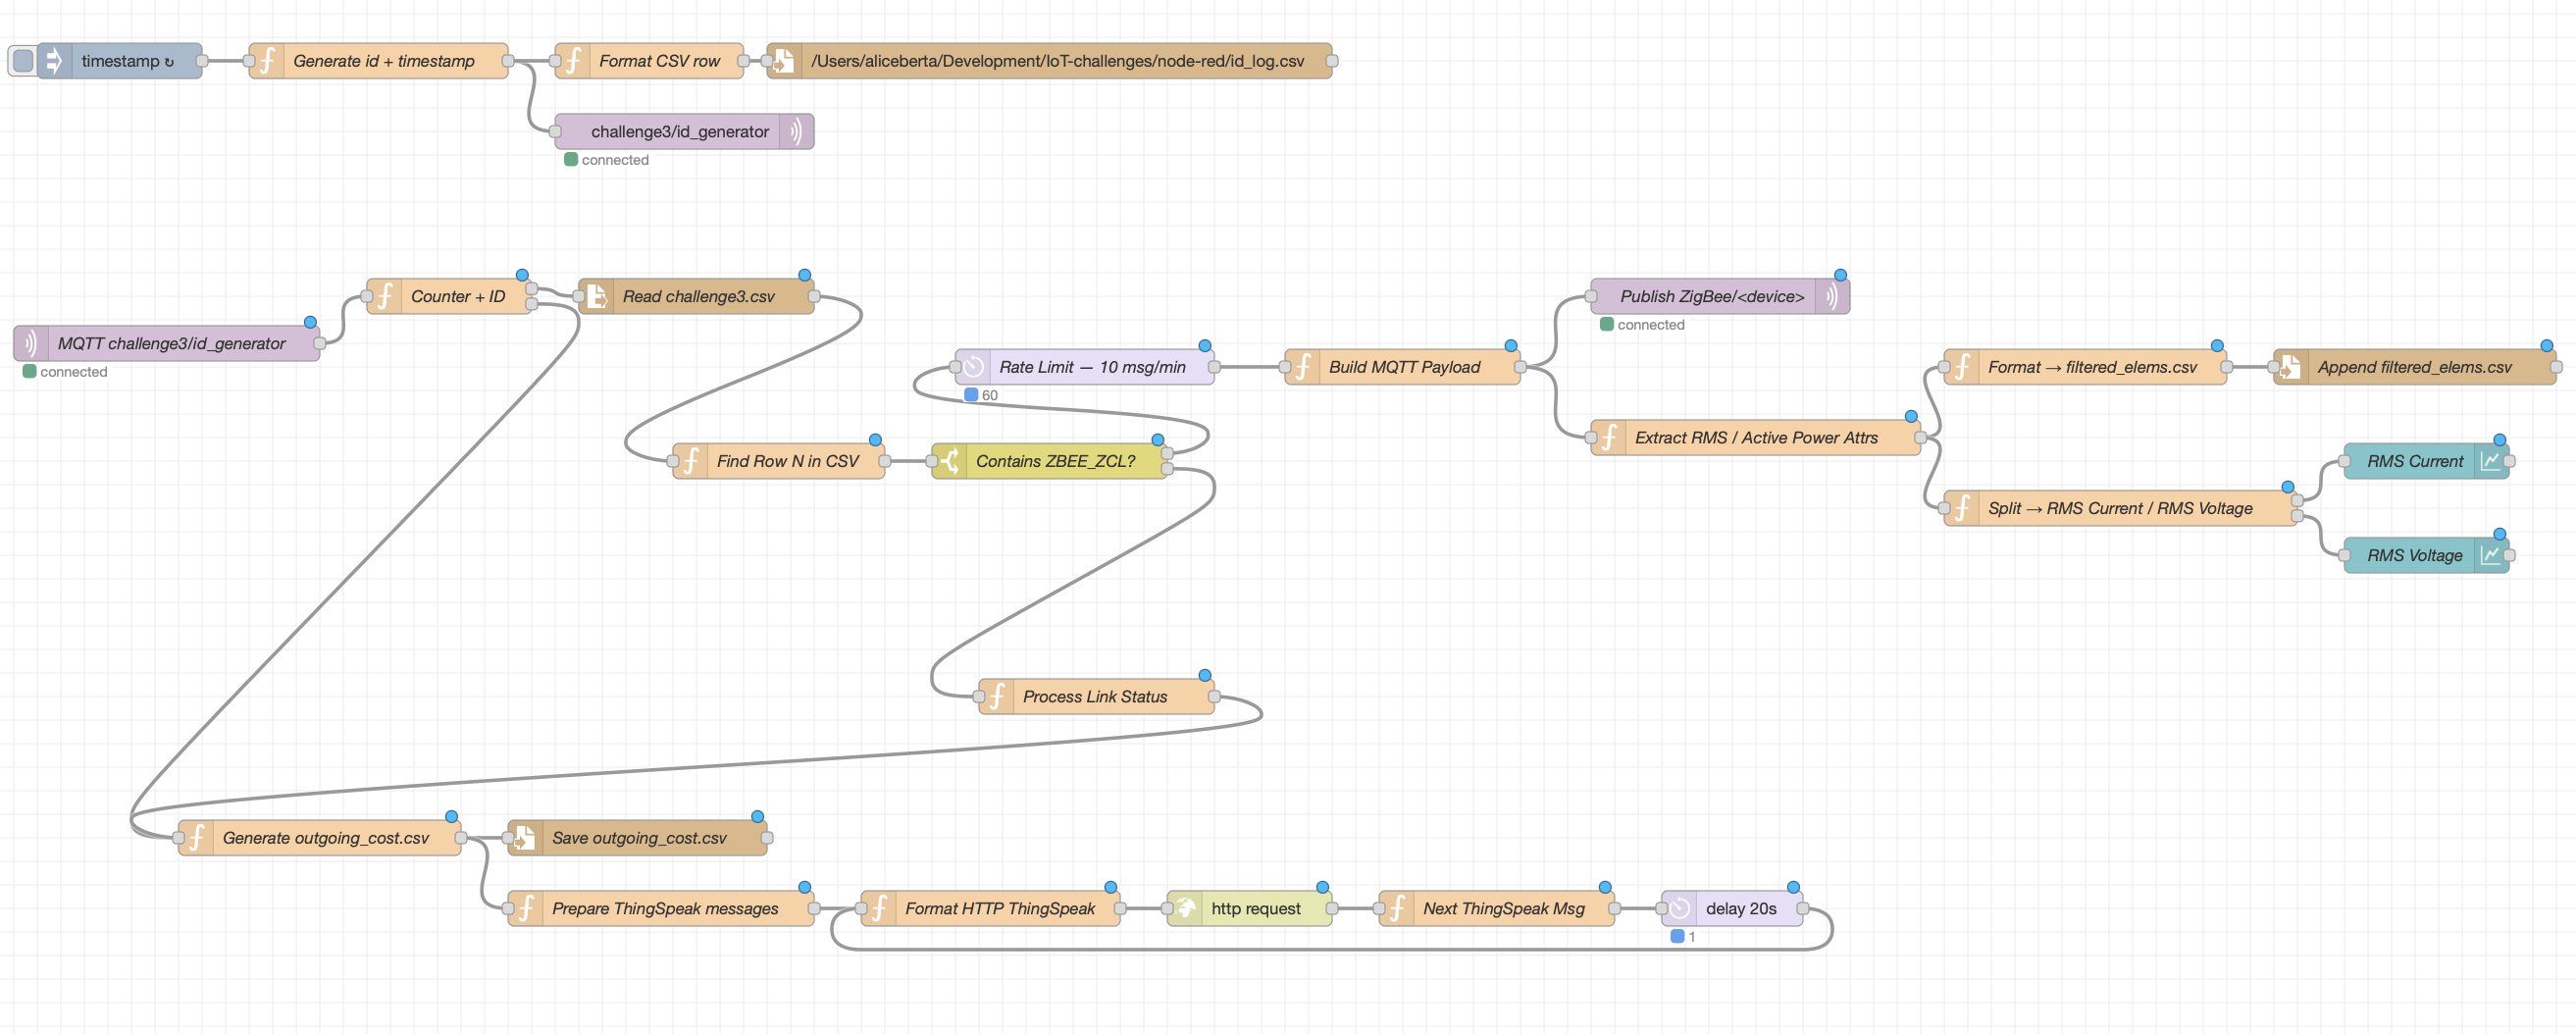
\includegraphics[width=\linewidth]{merged_flow.png}
    \caption{Complete flow.}
    \label{fig:complete-flow}
\end{figure}

The overall flow is composed of a single tab containing two main branches sharing the same MQTT broker (\texttt{localhost}, port \texttt{1884}):

\begin{itemize}
    \item \textbf{Publisher branch}: a periodic trigger generates a random ID and a UNIX timestamp, packages them as a JSON payload, publishes the message to the topic \texttt{challenge3/id\_generator}, and simultaneously writes the data to \texttt{id\_log.csv}.
    \item \textbf{Subscriber branch}: an MQTT-in node subscribes to the same topic, applies modulo arithmetic on the received ID to compute a packet index~\texttt{N}, reads the corresponding row from \texttt{challenge3.csv}, and dispatches the processing to one of three conditional paths depending on the packet type.
\end{itemize}

% ============================================================
\section{Task 1 -- Publisher Flow (1 point)}
% ============================================================

\subsection{Description}

The first task requires building a flow that periodically publishes an MQTT message to the local Mosquitto broker at \texttt{localhost:1884}, on the topic \texttt{challenge3/id\_generator}. Each message must carry a JSON payload containing two fields: a random integer \texttt{id} drawn uniformly in the range $[0, 30000]$, and a \texttt{timestamp} field representing the current UNIX time at the moment of generation. The publishing rate is fixed at one message per second. Additionally, every sent message must be logged to a CSV file named \texttt{id\_log.csv}, structured as \texttt{No.,ID,TIMESTAMP}, where \texttt{No.} is an incremental row counter.

\subsection{Implementation}

The publisher branch of the Node-RED flow was constructed to periodically generate data, publish it via MQTT, and log the records locally.

The first node is an \textbf{Inject node} called ``1s Trigger''. It acts as the primary clock for the flow, configured to fire automatically at a regular interval of 1 second.

The second node is a \textbf{Function node} called ``Generate ID + Timestamp''. Connected to the Inject node, it generates a random integer ID between 0 and 30,000 alongside the current UNIX timestamp. It then converts this object into a JSON-formatted string payload to ensure proper compatibility with the MQTT broker. The internal logic is implemented as follows:

\begin{lstlisting}[language=JavaScript, caption={Generate ID + Timestamp logic}]
msg.payload = {
    id: Math.floor(Math.random() * 30001),
    timestamp: Math.floor(Date.now() / 1000)
};
msg.payload = JSON.stringify(msg.payload);
return msg;
\end{lstlisting}

The third node is an \textbf{MQTT Out} node. Receiving the JSON string from the previous function, this node connects to the local Mosquitto broker at \texttt{localhost:1884} and publishes the payload to the \texttt{challenge3/id\_generator} topic.

The fourth node is a \textbf{Function node} called ``Format CSV row''. Branching off the data generation node, this block parses the JSON payload and uses a persistent context variable to maintain an incremental row counter. It formats the extracted data into a comma-separated string, adding the required header specifically for the first row. The code used is shown below:

\begin{lstlisting}[language=JavaScript, caption={Format CSV row logic}]
let count = context.get('count') || 0;
count++;
context.set('count', count);

const data = JSON.parse(msg.payload);

if (count === 1) {
    msg.payload = "No.,ID,TIMESTAMP\n" +
                  `${count},${data.id},${data.timestamp}\n`;
} else {
    msg.payload = `${count},${data.id},${data.timestamp}\n`;
}
return msg;
\end{lstlisting}

The fifth node is a \textbf{File node} called ``id\_log.csv''. Finally, this node receives the formatted CSV string and appends it to the local log file. The automatic newline feature is intentionally disabled to maintain the precise line break formatting established by the preceding function node.

\begin{figure}[H]
    \centering
    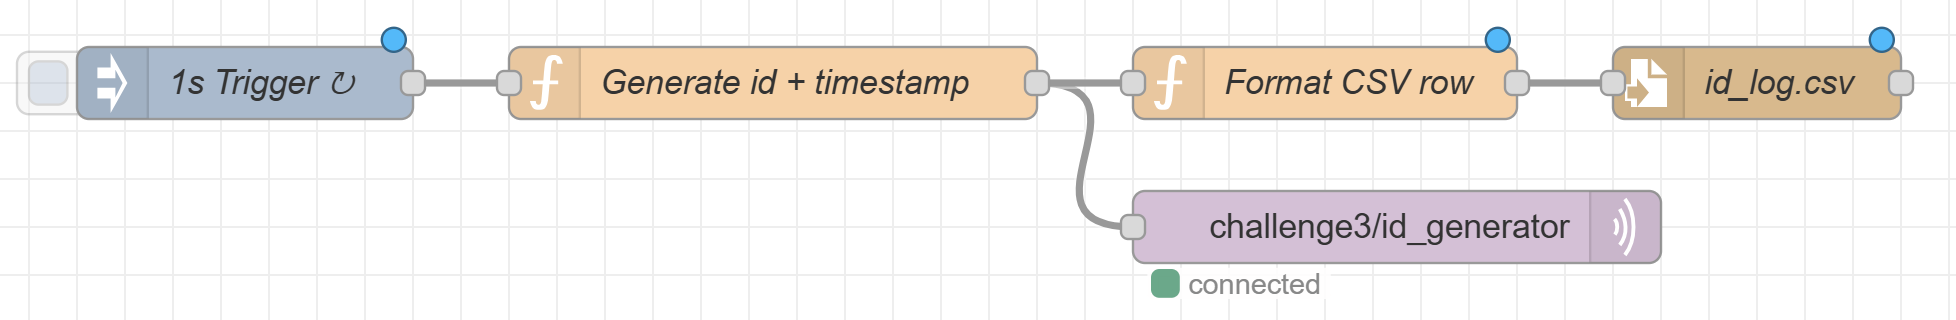
\includegraphics[width=\linewidth]{publisher_flow.png}
    \caption{Publisher flow.}
    \label{fig:pub-flow}
\end{figure}

\subsection{Output: \texttt{id\_log.csv}}

\begin{lstlisting}[caption={Excerpt of generated \texttt{id\_log.csv}.}]
No.,ID,TIMESTAMP
1,16320,1778573262
2,5225,1778573263
3,13278,1778573264
4,23212,1778573265
\end{lstlisting}

% ============================================================
\section{Task 2 -- Subscriber Branch with ZigBee Processing (2 points)}
% ============================================================

\subsection{Description}

The subscriber branch listens on the same \texttt{challenge3/id\_generator} topic. Each time a message arrives, the branch extracts the \texttt{id} field and uses it to compute a row index:
\[
    N = \texttt{id} \bmod 5218
\]
The row at position \texttt{N} in \texttt{challenge3.csv} is then fetched and inspected.

If its \texttt{Command String} column contains a \texttt{ZBEE\_ZCL} layer, the packet is published to a topic named after the ZigBee source device. The publish rate is capped at 10 messages per minute. When the published packet also carries \texttt{RMS Current}, \texttt{RMS Voltage}, or \texttt{Active Power} attributes, those values are extracted and appended to \texttt{filtered\_elems.csv}; the two electrical measurements are also plotted in real time on the Node-Red dashboard.

Packets that do not contain \texttt{ZBEE\_ZCL} are silently discarded. The branch stops after exactly 200 messages have been received, whether or not each message produced a publishable packet.

\subsection{Implementation}

The subscriber branch is a linear chain of function and utility nodes. Each node passes its result forward; returning \texttt{null} at any point stops that message immediately.

During development, the external MQTT publisher was not yet available. To allow independent testing, the MQTT-in node was temporarily replaced by an \textbf{Inject node} configured to fire every second. The random \texttt{id} and UNIX timestamp were generated inside the \textit{Counter + ID} function node itself. Switching to the real MQTT subscriber requires only reconnecting the wire from the Inject node to the MQTT-in node; no other change to the flow is needed.

\subsubsection*{Node 1 — Counter + ID}

This function node is the entry point of the subscriber branch and has two outputs. Its first job is to maintain a running count of messages processed so far, stored in \texttt{flow.get('msgCount')}. If the count has already exceeded 200, the node logs a warning and returns \texttt{null}, dropping the message silently.

\begin{lstlisting}[language=JavaScript, caption={Counter + ID -- function node.}]
var count = flow.get('msgCount') || 0;
count++;
if (count > 200) {
    node.warn('200-message limit reached -- stopping.');
    return null;
}
flow.set('msgCount', count);

var id, ts;
if (msg.payload && typeof msg.payload === 'object' &&
        msg.payload.id !== undefined) {
    id = Number(msg.payload.id);
    ts = Number(msg.payload.timestamp);
} else {
    id = Math.floor(Math.random() * 30001);
    ts = Math.floor(Date.now() / 1000);
}

msg.subId    = id;
msg.subTs    = ts;
msg.N        = id % 5218;
msg.msgCount = count;
msg.filename = flow.get('csvPath') ||
    '/Users/aliceberta/Development/IoT-challenges/node-red/challenge3.csv';

if (count === 200) {
    node.send([msg, { payload: 'save' }]);
    return null;
}
return msg;
\end{lstlisting}

If the limit has not been reached, the node reads \texttt{id} and \texttt{timestamp} from the JSON payload delivered by the MQTT broker. The row index \texttt{N} is computed as \texttt{id~mod~5218} and the path to the CSV file is attached to the message. The current count is also stored in \texttt{msg.msgCount} for reference by downstream nodes. When the count reaches exactly 200, the node fires a trigger message on its second output (\texttt{\{payload: 'save'\}}) to initiate the final dump of \texttt{outgoing\_cost.csv}, then stops processing by returning \texttt{null}.

\subsubsection*{Node 2 — Read challenge3.csv}

A \textbf{File In} node reads the entire content of \texttt{challenge3.csv} as a UTF-8 string into \texttt{msg.payload}. The file path is taken dynamically from \texttt{msg.filename}, so no path is hard-coded inside the node configuration. All properties set by the previous node (\texttt{msg.N}, \texttt{msg.subId}, etc.) are preserved across the read.

\subsubsection*{Node 3 — Find Row N}

The built-in CSV node is not used here because the \texttt{Command String} column contains commas inside quoted substrings, which would break a simple split. A custom character-by-character parser handles quoted fields correctly.

\begin{lstlisting}[language=JavaScript, caption={Find Row N -- function node.}]
var N       = msg.N;
var csvText = msg.payload;

function parseLine(line) {
    var res = [], field = '', inQ = false;
    for (var i = 0; i < line.length; i++) {
        var c = line[i];
        if (c === '"')              { inQ = !inQ; }
        else if (c === ',' && !inQ) { res.push(field.trim()); field = ''; }
        else                        { field += c; }
    }
    res.push(field.trim());
    return res;
}

var lines   = csvText.split('\n');
var headers = parseLine(lines[0]);

for (var i = 1; i < lines.length; i++) {
    if (!lines[i].trim()) continue;
    var fields = parseLine(lines[i]);
    if (parseInt(fields[0]) === N) {
        var row = {};
        headers.forEach(function(h, j) { row[h] = fields[j] || ''; });
        msg.row        = row;
        msg.commandStr = row['Command String'] || '';
        return msg;
    }
}
node.warn('Packet N=' + N + ' not found in CSV -- skipping');
return null;
\end{lstlisting}

The parser flips a boolean flag \texttt{inQ} each time it meets a double-quote character, and only splits on commas found while \texttt{inQ} is \texttt{false}. Once the matching row is located, its fields are stored as a key-value object in \texttt{msg.row} and the command string is copied into \texttt{msg.commandStr} for downstream nodes. If no row matches, a warning is logged and the message is dropped.

\subsubsection*{Node 4 — ZBEE\_ZCL?}

A \textbf{Switch} node checks whether \texttt{msg.commandStr} contains the substring \texttt{ZBEE\_ZCL}. Only messages that satisfy this condition are forwarded; all others are silently dropped. This single check filters out Link Status frames and any other protocol that is not a ZigBee Cluster Library packet.

\subsubsection*{Node 5 — Max 10 msg/min}

A \textbf{Delay} node configured in \textit{Rate Limit} mode ensures that no more than 10 messages per minute are forwarded to the publish stage. Messages that arrive faster than this rate are queued and released gradually; none are dropped.

\subsubsection*{Node 6 — Build MQTT Payload}

This function node assembles the JSON payload required by the specification and sets the dynamic MQTT topic.

\begin{lstlisting}[language=JavaScript, caption={Build MQTT payload -- function node.}]
var row = msg.row;
var deviceName = (row['Device Name ZigBee Source'] || 'unknown')
    .trim()
    .replace(/[^a-zA-Z0-9\s\-_]/g, '')
    .trim() || 'unknown';

var payload = {
    timestamp  : Math.floor(Date.now() / 1000),
    id         : msg.subId,
    'wpan.src' : row['Source Address']             || '',
    'wpan.dst' : row['Destination Address']        || '',
    'zbee.src' : row['Source Address ZigBee']      || '',
    'zbee.dst' : row['Destination Address ZigBee'] || '',
    topic      : 'ZigBee/' + deviceName,
    payload    : msg.commandStr
};

msg.topic      = 'ZigBee/' + deviceName;
msg.payload    = JSON.stringify(payload);
msg.pubTs      = payload.timestamp;
msg.deviceName = deviceName;
return msg;
\end{lstlisting}

The device name is read from the \texttt{Device Name ZigBee Source} column and sanitised with a regular expression that removes any character that would be invalid in an MQTT topic path. The assembled payload is serialised to JSON and placed in \texttt{msg.payload}; the topic string is stored in \texttt{msg.topic} so that the MQTT Out node can pick it up dynamically. The publish timestamp is also saved as \texttt{msg.pubTs} for use by the CSV writer downstream.

From the output of \textit{Build MQTT Payload} two wires depart in parallel. The first connects to an \textbf{MQTT Out} node that publishes the assembled payload to \texttt{localhost:1884} on the dynamic topic stored in \texttt{msg.topic}. The second wire leads to the \textit{Extract RMS / Active Power Attrs} function node.

\subsubsection*{Node 7 — Extract RMS / Active Power Attrs}

The \texttt{Command String} field is formatted as a Python dictionary with single-quoted keys and values. The \texttt{parsePyDict} helper converts it to valid JSON before parsing.

\begin{lstlisting}[language=JavaScript, caption={Extract RMS / Active Power Attrs -- function node.}]
var cmdStr = msg.commandStr;

function parsePyDict(s) {
    s = s.replace(/'/g, '"');
    s = s.replace(/\bNone\b/g, 'null');
    s = s.replace(/\bTrue\b/g, 'true');
    s = s.replace(/\bFalse\b/g, 'false');
    try { return JSON.parse(s); } catch(e) {
        node.warn('Parse error: ' + e.message);
        return null;
    }
}

var d = parsePyDict(cmdStr);
if (!d)          { return null; }
if (!d['Status']){ return null; }

function toArr(v) { return v === undefined ? [] : [].concat(v); }

var attrs     = toArr(d['Attribute']);
var stats     = toArr(d['Status']);
var dtypes    = toArr(d['Data Type']);
var seqNum    = d['Sequence Number'] || '';
var int16Arr  = toArr(d['Int16']);
var uint16Arr = toArr(d['Uint16']);
var int16i = 0, uint16i = 0;

var TARGETS = ['RMS Current', 'RMS Voltage', 'Active Power'];
var found = [];

for (var i = 0; i < attrs.length; i++) {
    var attrName  = (attrs[i]  + '').split(' (')[0].trim();
    var statusStr = (stats[i]  + '').split(' (')[0].trim();
    var dtypeStr  = (dtypes[i] + '').split(' (')[0].trim();
    var dtype     = dtypeStr.toLowerCase();
    var val = '';

    if (dtype.includes('signed') && !dtype.includes('unsigned'))
        val = (int16Arr[int16i++]  + '').split(' (')[0].trim();
    else if (dtype.includes('unsigned'))
        val = (uint16Arr[uint16i++] + '').split(' (')[0].trim();

    if (TARGETS.some(function(t) { return attrName.includes(t); }))
        found.push({ attribute: attrName, status: statusStr,
                     dataType: dtypeStr, value: val, seqNum: seqNum });
}

if (found.length === 0) { return null; }
msg.filteredAttrs = found;
return msg;
\end{lstlisting}

Only \textit{Read Attributes Response} packets contain both a \texttt{Status} and numeric value arrays; packets without a \texttt{Status} key are discarded immediately. The helper \texttt{toArr} wraps a single value in an array so that the loop works identically whether the CSV field holds one attribute or many. Because the CSV stores signed integers under the key \texttt{Int16} and unsigned integers under \texttt{Uint16}, the correct counter (\texttt{int16i} or \texttt{uint16i}) is incremented for every attribute visited, preserving positional alignment even for attributes that are not in the target list. Attribute names, status strings, and data type labels are truncated at the first space-parenthesis sequence (\texttt{split(' (')[0]}) to strip the numeric code appended by Wireshark.

From \textit{Extract RMS / Active Power Attrs} two further wires depart in parallel: one leads to the CSV writer chain, the other to the chart splitter.

\subsubsection*{Node 8 — Format filtered\_elems.csv}

\begin{lstlisting}[language=JavaScript, caption={Format filtered\_elems.csv -- function node.}]
var ts    = msg.pubTs || Math.floor(Date.now() / 1000);
var count = flow.get('filteredCount') || 0;
var lines = [];

msg.filteredAttrs.forEach(function(item) {
    count++;
    lines.push([count, ts, item.seqNum, item.attribute,
                item.status, item.dataType, item.value].join(','));
});
flow.set('filteredCount', count);

var out = '';
if (!flow.get('filteredHeader')) {
    out = 'No.,Timestamp,Sequence Number,Attribute,' +
          'Status,Data Type,Data Value\n';
    flow.set('filteredHeader', true);
}
out += lines.join('\n') + '\n';

msg.payload = out;
return msg;
\end{lstlisting}

A flow-scoped counter keeps the row numbers consistent across multiple messages. The CSV header is written exactly once, the first time this node executes, controlled by the boolean flag \texttt{filteredHeader}. The output is then appended to \texttt{filtered\_elems.csv} by a \textbf{File Out} node configured in append mode with automatic newlines disabled.

\subsubsection*{Node 9 — Chart Split}

\begin{lstlisting}[language=JavaScript, caption={Chart Split -- function node (2 outputs).}]
var currentMsg = null;
var voltageMsg = null;

msg.filteredAttrs.forEach(function(item) {
    var numVal = parseFloat(item.value);
    if (isNaN(numVal)) numVal = 0;

    if (item.attribute.includes('RMS Current'))
        currentMsg = { payload: numVal, topic: 'RMS Current' };
    else if (item.attribute.includes('RMS Voltage'))
        voltageMsg = { payload: numVal, topic: 'RMS Voltage' };
});

return [currentMsg, voltageMsg];
\end{lstlisting}

This two-output function node separates RMS Current and RMS Voltage into independent messages. Output~0 feeds the RMS Current chart and output~1 feeds the RMS Voltage chart on the Node-Red dashboard. Active Power is not plotted and is therefore ignored here. If a particular attribute is absent from the current message, the corresponding output remains \texttt{null} and no message is sent to that chart.

\begin{figure}[H]
    \centering
    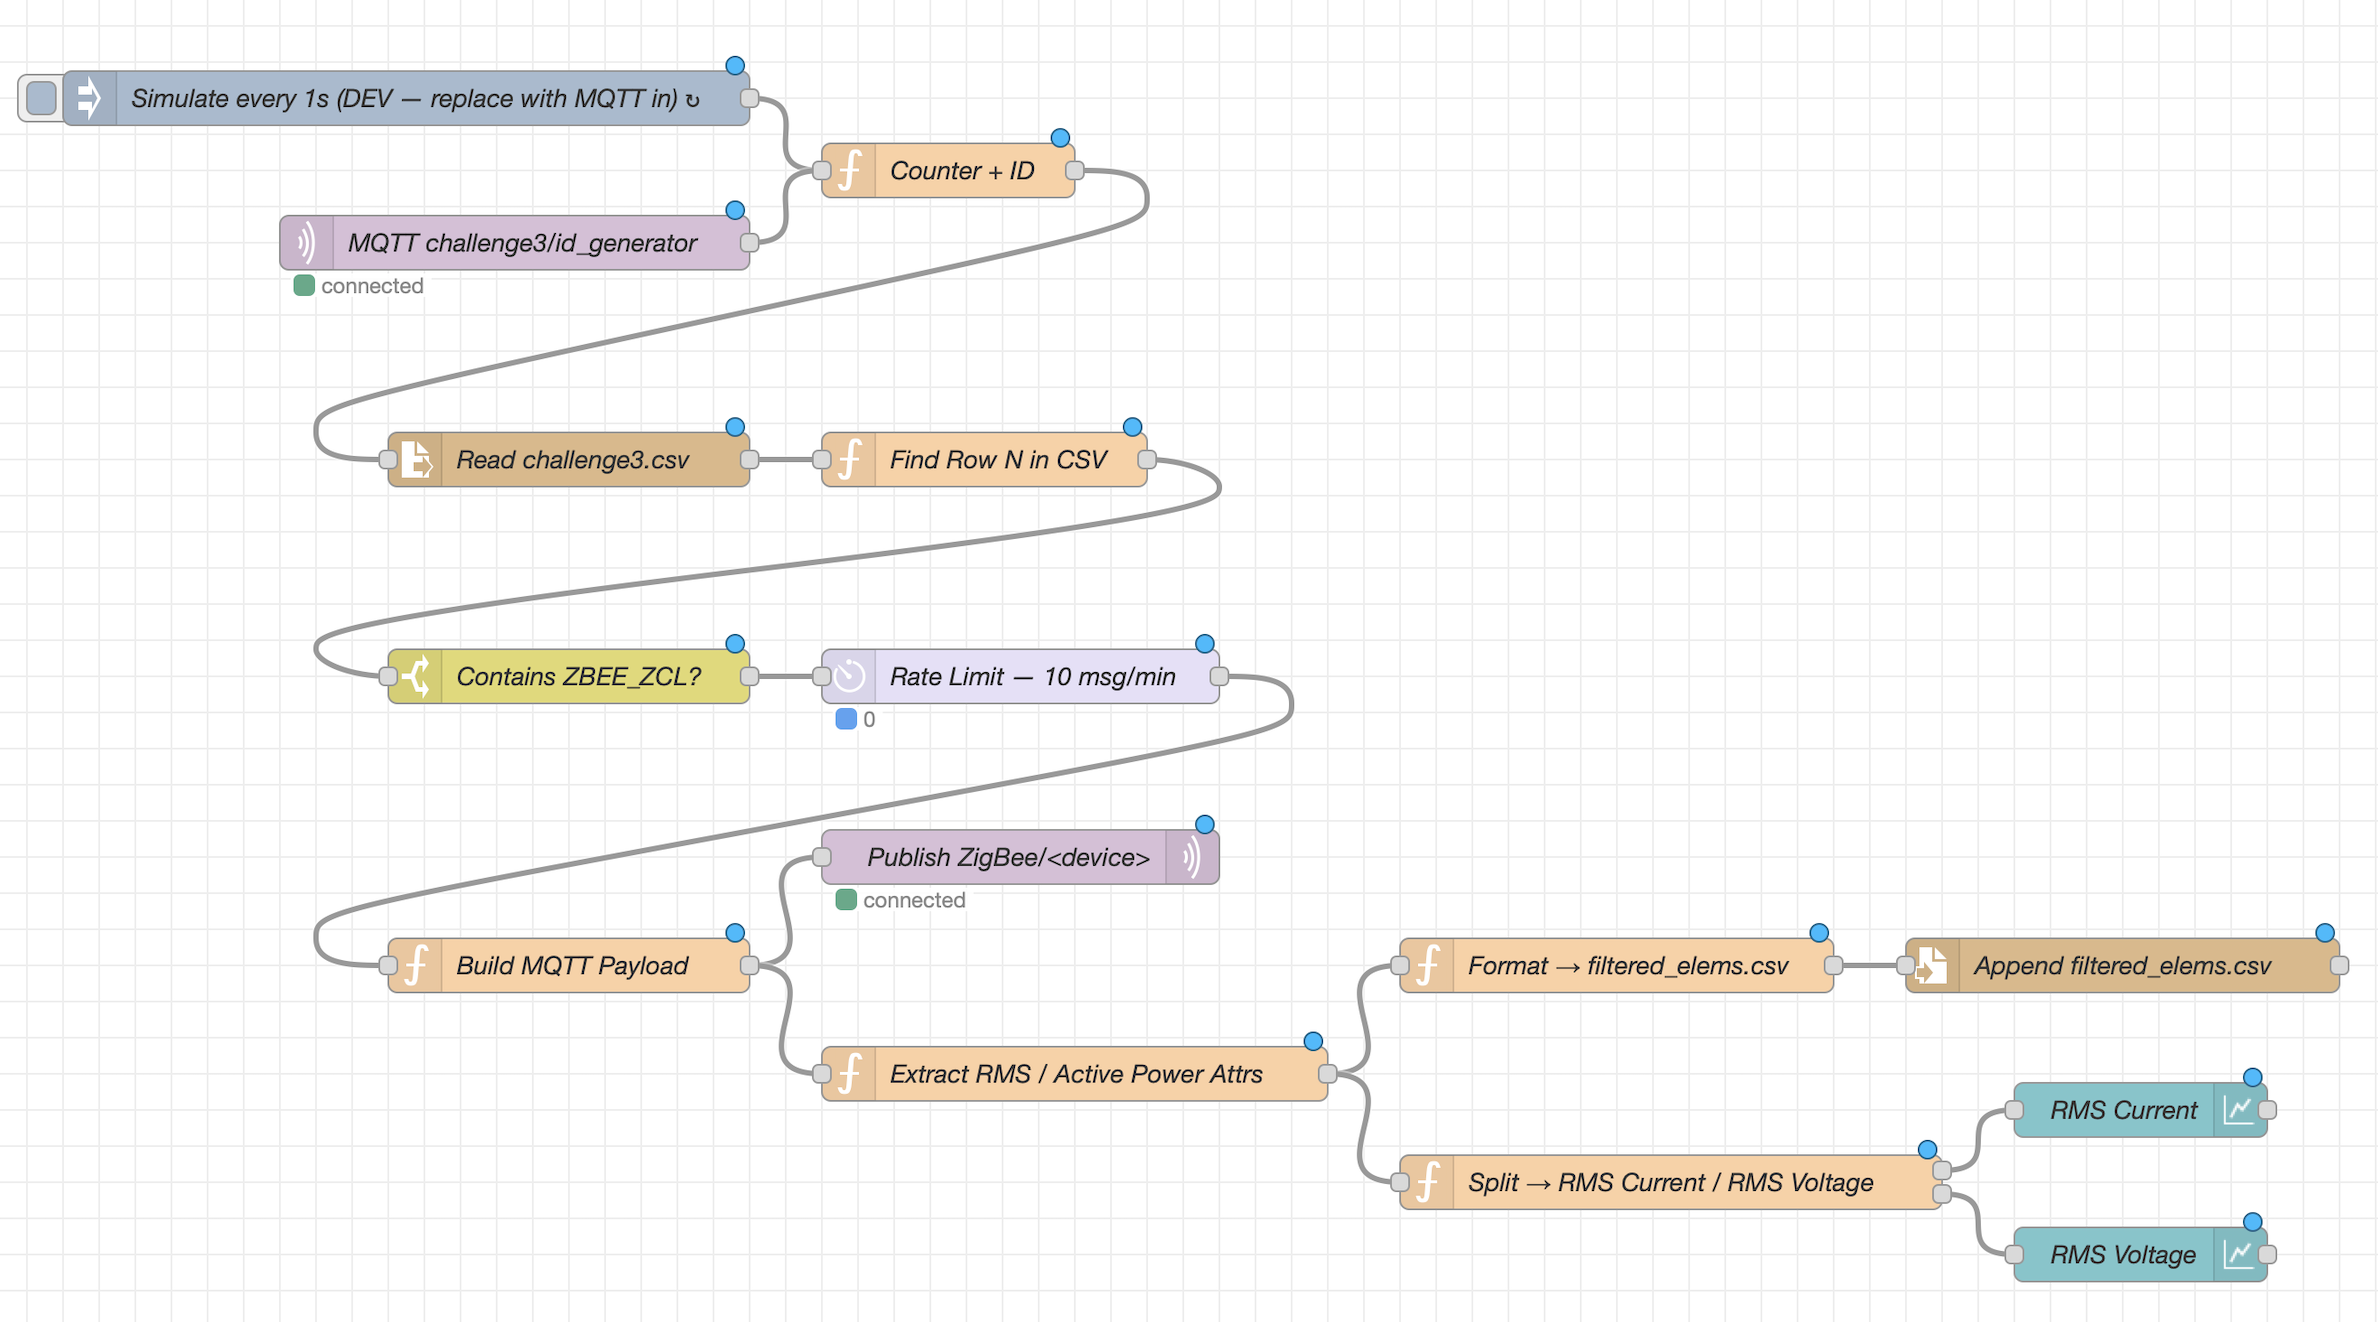
\includegraphics[width=0.95\textwidth]{subscriber_flow.png}
    \caption{Subscriber flow.}
    \label{fig:sub-flow}
\end{figure}

\subsection{MQTT Publish Payload Format}

When a \texttt{ZBEE\_ZCL} layer is detected, the message published to \texttt{ZigBee/<ZB\_SRC\_DEV\_NAME>} uses the following JSON structure:

\begin{lstlisting}[language={}]
{
  "timestamp": CURRENT_TIMESTAMP,
  "id": SUB_ID,
  "wpan.src": "SRC_ADDR",
  "wpan.dst": "DST_ADDR",
  "zbee.src": "ZB_SRC_ADDR",
  "zbee.dst": "ZB_DST_ADDR",
  "topic": "ZigBee/ZB_SRC_DEV_NAME",
  "payload": CMD_STR
}
\end{lstlisting}

All address fields are in hexadecimal format (e.g., \texttt{0x1cd8}). \texttt{SUB\_ID} is the original \texttt{id} value received from the subscription (before the modulo), and \texttt{CURRENT\_TIMESTAMP} is the UNIX time at the moment the publish message is sent.

\subsection{Output: \texttt{filtered\_elems.csv}}

\begin{lstlisting}[caption={Excerpt of generated \texttt{filtered\_elems.csv}.}]
No.,Timestamp,Sequence Number,Attribute,Status,Data Type,Data Value
1,1778573280,245,Active Power,Success,16-Bit Signed Integer,0
2,1778573280,245,RMS Current,Success,16-Bit Unsigned Integer,0
3,1778573280,245,RMS Voltage,Success,16-Bit Unsigned Integer,219
\end{lstlisting}

\subsection{Node-Red Dashboard Charts}

The RMS Current and RMS Voltage values are displayed in real time on two separate line charts on the Node-Red dashboard, accessible at \url{http://localhost:1880/ui}. The dashboard was built using the \texttt{@flowfuse/node-red-dashboard} package. Both charts belong to the group \textit{Electrical Measurements} inside the page \textit{ZigBee Monitor}.

\begin{figure}[H]
    \centering
    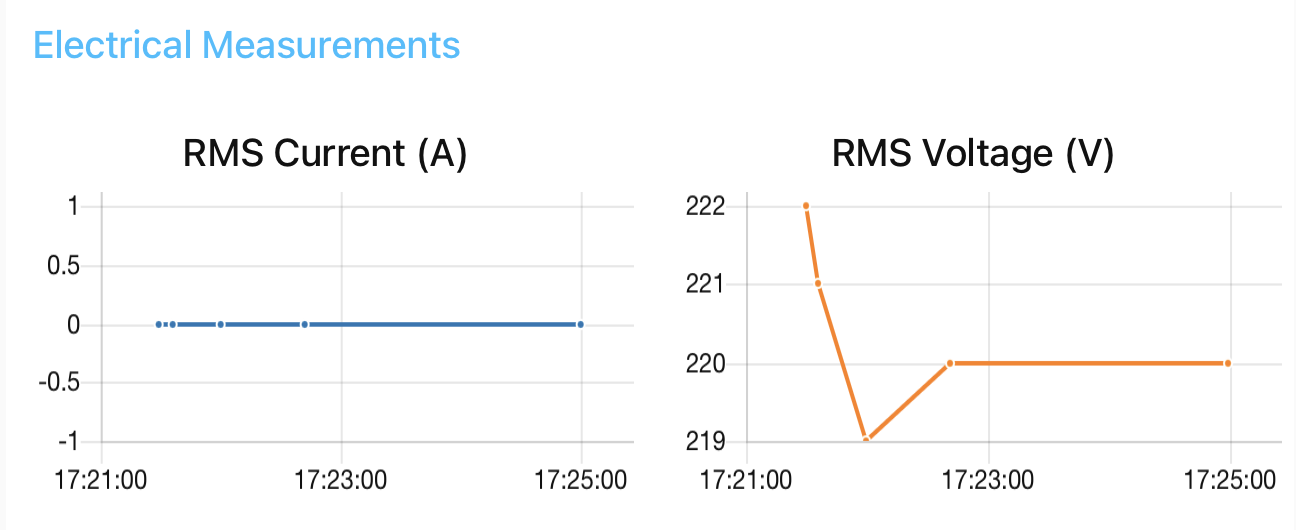
\includegraphics[width=0.95\textwidth]{dashboard.png}
    \caption{Node-Red dashboard showing real-time RMS Current (left) and RMS Voltage (right) charts.}
    \label{fig:dashboard}
\end{figure}

% ============================================================
\section{Task 3 -- Link Status Handling and ThingSpeak Publishing (2 points)}
% ============================================================

\subsection{Description}

When the packet retrieved from \texttt{challenge3.csv} at index~\texttt{N} is a Link Status packet (i.e., the command string contains \texttt{Link Status (0x08)}), the flow extracts the outgoing cost for each link associated with the ZigBee source address. If a later Link Status packet arrives from the same source address, the stored costs are updated. At the end of the execution (after 200 ID messages have been processed), all collected link costs are saved to \texttt{outgoing\_cost.csv} with the format \texttt{No., Source, Destination, Cost}.

Subsequently, the smallest source address in \texttt{outgoing\_cost.csv} (treating addresses as hexadecimal integers) is identified. Its destination addresses are sorted in ascending hexadecimal order, and the corresponding outgoing costs are sent one by one to a public ThingSpeak channel via the HTTP API, placing each cost value in \texttt{field1}. Messages are sent in destination-address order with a rate limit of one message every 20 seconds.

\subsection{Implementation}

This branch processes incoming MQTT messages to detect Link Status packets, maintains a running table of outgoing costs in flow context, and at the 200-message limit dumps the results to a CSV file and uploads them to ThingSpeak.

\subsubsection*{Node 1 — Process Link Status}

This function node extracts the outgoing cost for every neighbour listed in the Link Status packet and stores the results in a flow-context object (\texttt{flow.costTable}) keyed by ZigBee source address. If a later packet arrives from the same source address, its entries overwrite the previously stored values, implementing the update semantics required by the specification.

Because the \texttt{Command String} field uses Python-style single-quoted dictionaries rather than valid JSON, the node uses a regular expression to extract each link entry without attempting a full JSON parse.

\begin{lstlisting}[language=JavaScript, caption={Process Link Status}]
const packetType = msg.row['Packet Type'] || '';

if (!packetType.includes('Link Status (0x08)')) {
    return null;
}

let costTable = flow.get('costTable') || {};

const source  = msg.row['Source Address ZigBee'].trim();
const cmdStr  = msg.row['Command String'];

// Extract link entries with a regex (command string is Python-like,
// not valid JSON, so JSON.parse cannot be used directly)
const linkRegex =
    /\{'Address':\s*'(0x[0-9a-fA-F]+)',\s*'Incoming Cost':\s*'\d+',\s*'Outgoing Cost':\s*'(\d+)'\}/g;

let match;
costTable[source] = costTable[source] || {};

while ((match = linkRegex.exec(cmdStr)) !== null) {
    const address      = match[1];
    const outgoingCost = match[2];
    costTable[source][address] = outgoingCost;
}

flow.set('costTable', costTable);

return null;
\end{lstlisting}

\textbf{Connections:} no output (returns \texttt{null} always); the cost table is updated in flow context as a side effect.

% ------------------------------------------------------------
\subsubsection*{Node 2 — Generate outgoing\_cost.csv}

Triggered by the second output of \textit{Counter + ID} when the 200-message limit is reached. It reads \texttt{flow.costTable}, serialises every source--destination--cost triple into CSV rows, and sets \texttt{msg.payload} to the full file content (including the header line).

\begin{lstlisting}[language=JavaScript, caption={Generate outgoing\_cost.csv}]
const costTable = flow.get('costTable') || {};

let rows = ['No.,Source,Destination,Cost'];
let rowNum = 1;

const sources = Object.keys(costTable);
sources.forEach(source => {
    const destinations = Object.keys(costTable[source]);
    destinations.forEach(dest => {
        const cost = costTable[source][dest];
        rows.push(`${rowNum},${source},${dest},${cost}`);
        rowNum++;
    });
});

msg.payload = rows.join('\n');
return msg;
\end{lstlisting}

\textbf{Connections:} output $\to$ \textit{Save outgoing\_cost.csv} and $\to$ \textit{Prepare ThingSpeak Messages}.

\subsubsection*{Node 3 — Save outgoing\_cost.csv}

A built-in \textit{write file} node configured to overwrite the file at the specified path with the content of \texttt{msg.payload}. The newline option is disabled because line endings are already embedded in the payload string.

\textbf{Connections:} no further output.

\subsubsection*{Node 4 — Prepare ThingSpeak Messages}

Reads \texttt{flow.costTable}, finds the source address with the smallest hexadecimal value, sorts its destination addresses in ascending hexadecimal order, and stores the ordered list of \{cost, destination, source\} objects in \texttt{flow.thingspeakMessages}. It then emits the first message immediately.

\begin{lstlisting}[language=JavaScript, caption={Prepare ThingSpeak Messages}]
const costTable = flow.get('costTable') || {};

// Find the source with the smallest hex address
const sources = Object.keys(costTable);
const smallestSource = sources.sort((a, b) =>
    parseInt(a, 16) - parseInt(b, 16)
)[0];

// Sort destinations in ascending hex order
const destinations = Object.keys(costTable[smallestSource]);
destinations.sort((a, b) => parseInt(a, 16) - parseInt(b, 16));

const messages = destinations.map(dest => ({
    cost:        costTable[smallestSource][dest],
    destination: dest,
    source:      smallestSource
}));

flow.set('thingspeakMessages', messages);
flow.set('thingspeakIndex', 0);

msg.payload = messages[0];
return msg;
\end{lstlisting}

\textbf{Connections:} output $\to$ \textit{Format HTTP ThingSpeak}.

% ------------------------------------------------------------
\subsubsection*{Node 5 — Format HTTP ThingSpeak}

Builds the ThingSpeak HTTP GET URL by injecting the outgoing cost into the \texttt{field1} query parameter together with the channel Write API Key.

\begin{lstlisting}[language=JavaScript, caption={Format HTTP ThingSpeak}]
const WRITE_API_KEY = 'OUR_API_KEY';
const cost = msg.payload.cost;

msg.url    = `https://api.thingspeak.com/update?api_key=${WRITE_API_KEY}&field1=${cost}`;
msg.method = 'GET';

return msg;
\end{lstlisting}

\textbf{Connections:} output $\to$ \textit{HTTP Request}.

% ------------------------------------------------------------
\subsubsection*{Node 6 — HTTP Request}

A built-in \textit{http request} node configured to perform a GET request to the URL stored in \texttt{msg.url}. The response is returned as a UTF-8 string. A successful update returns the entry ID assigned by ThingSpeak.

\textbf{Connections:} output $\to$ \textit{Next ThingSpeak Message}.

% ------------------------------------------------------------
\subsubsection*{Node 7 — Next ThingSpeak Message}

After each successful HTTP request this node increments the index into the message list and emits the next message, or stops the loop when all destinations have been uploaded.

\begin{lstlisting}[language=JavaScript, caption={Next ThingSpeak Message}]
const messages = flow.get('thingspeakMessages') || [];
let index = flow.get('thingspeakIndex') || 0;
index++;
flow.set('thingspeakIndex', index);

if (index >= messages.length) {
    node.warn('ThingSpeak: all messages sent!');
    return null;
}

msg.payload = messages[index];
return msg;
\end{lstlisting}

\textbf{Connections:} output $\to$ \textit{Delay 20s}.

% ------------------------------------------------------------
\subsubsection*{Node 8 — Delay 20s}

A built-in \textit{delay} node set to delay each message by exactly 20 seconds, enforcing the rate limit of one ThingSpeak update per 20 seconds required by the specification.

\textbf{Connections:} output $\to$ \textit{Format HTTP ThingSpeak} (closes the loop).

\begin{figure}[H]
    \centering
    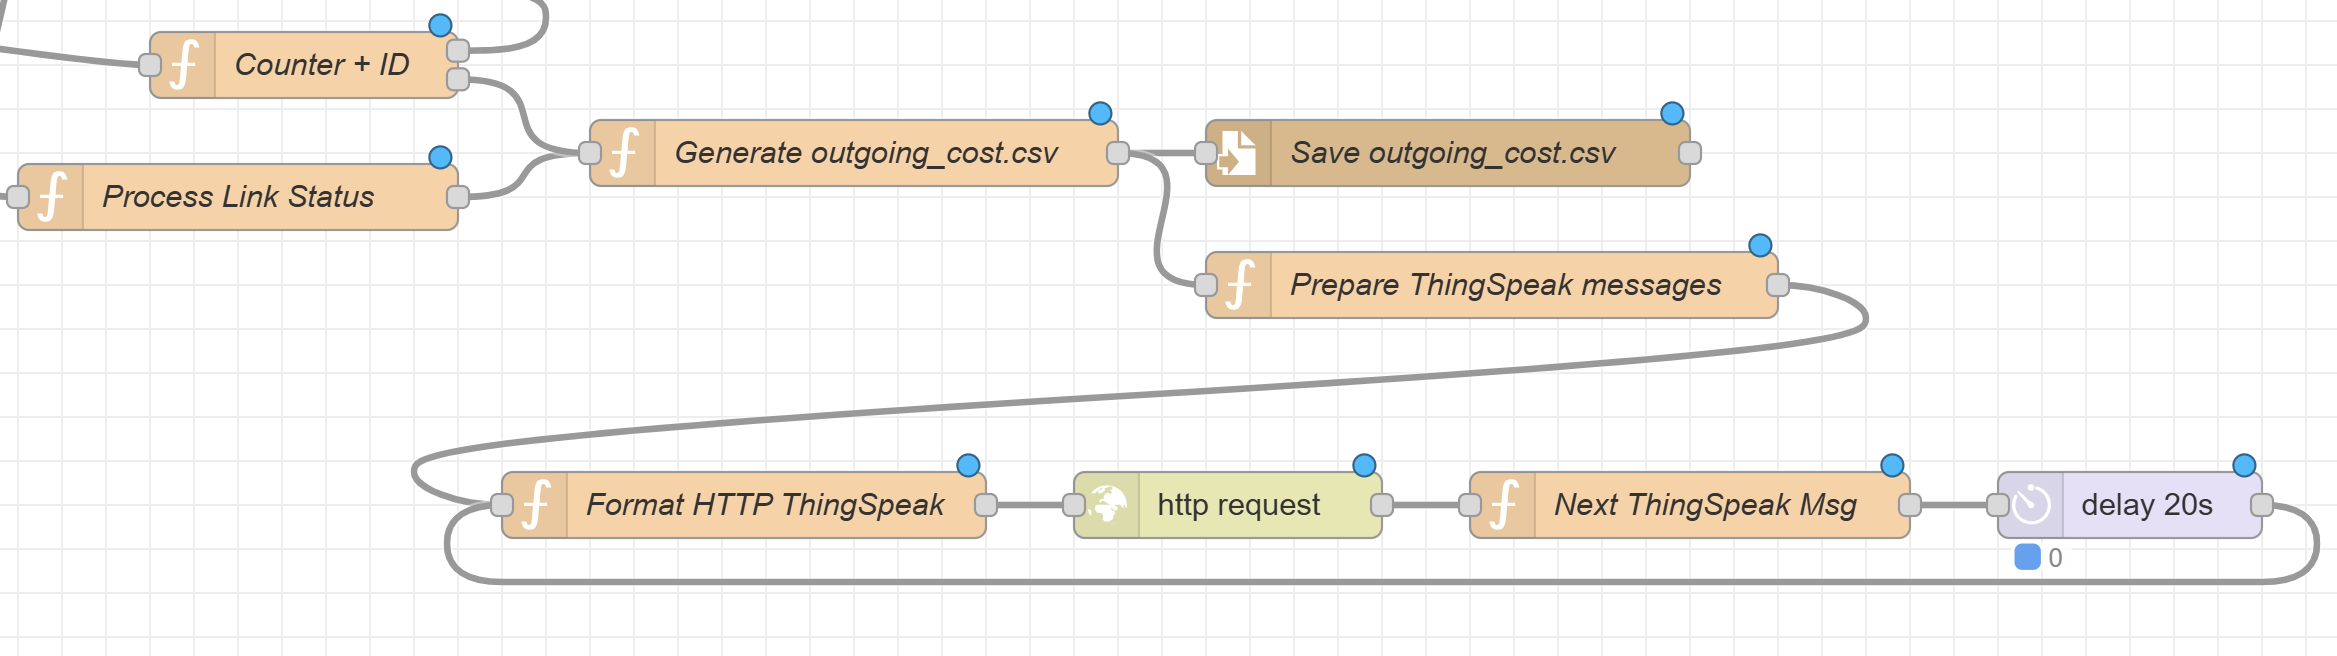
\includegraphics[width=\linewidth]{link_status_flow.png}
    \caption{Link Status branch flow.}
    \label{fig:link-status-flow}
\end{figure}

\subsection{Output: \texttt{outgoing\_cost.csv}}

\begin{lstlisting}[caption={Excerpt of generated \texttt{outgoing\_cost.csv}.}]
No.,Source,Destination,Cost
1,0x1cd8,0x0000,1
2,0x1cd8,0x0112,3
3,0x1cd8,0x1e15,1
4,0x1cd8,0x3d95,1
5,0x1cd8,0x4e11,3
\end{lstlisting}

\subsection{ThingSpeak Channel}

\begin{center}
    \url{https://thingspeak.mathworks.com/channels/3378810}
\end{center}

\begin{figure}[H]
    \centering
    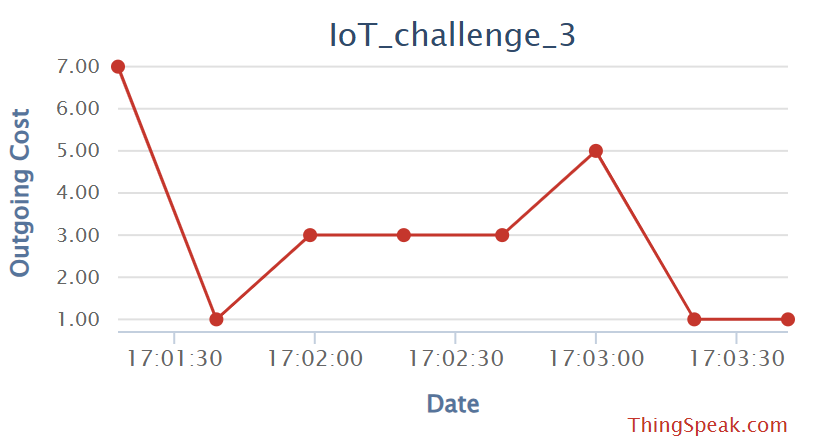
\includegraphics[width=0.5\linewidth]{outgoing_cost.png}
    \caption{Outgoing costs in ThingSpeak.}
    \label{fig:thingspeak}
\end{figure}

\end{document}